\documentclass{article}
\usepackage{tabularx,ragged2e,booktabs,caption}
\usepackage{graphicx}
\usepackage{float}

\title{Assignment 1}
\author{Francesco Andreuzzi}
\date{\today}

\begin{document}
\maketitle

\section{MPI Programming}

\subsection{Ring}

\subsubsection{Implementation}
I implemented in C++ a ring with the given characteristics. Communications are carried out using the asynchronous operations \texttt{MPI\_Isend, MPI\_Irecv}, after two input communications and two output communications on a given process the function \texttt{MPI\_Waitall} is called in order to wait for the communication to be completed. The time is measured on the process \texttt{rank0}, and I called \texttt{MPI\_Barrier} just before measuring the elapsed time in order to wait for all the other processes to receive their initial messages, which for my understanding of the problem represents the total time. Since the times I measured are quite small I repeated the experiment about 10000 times for all the parameters available.

\subsubsection{Analysis}
In Figure \ref{fig:ring_performance} we report the performance of \texttt{ring.cpp} for varying number of processors. We expect an approximately linear growth, since the addition of a new process introduces a new step in the ring (and therefore two more input and two output messages for each process).

\begin{figure}[t]
    \centering
    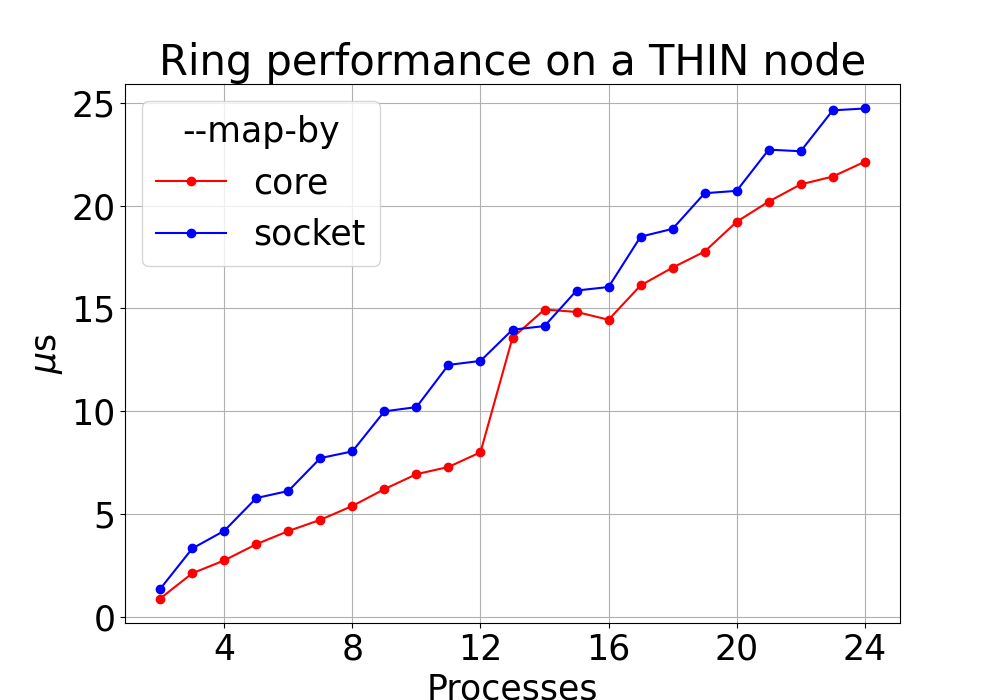
\includegraphics[width=\textwidth]{ring/fig.png}
    \caption{The script (written in C++) has been run multiple times ($\sim$ 10000) on a THIN node. Output was disabled via a compiler flag while taking times, in order to avoid polluting measurements.}
    \label{fig:ring_performance}
\end{figure}

The time is taken for two values of \texttt{--map-by}, namely \texttt{core} and \texttt{socket}. As expected the \texttt{--map-by core} case outperforms the other one until \texttt{P=13}. As soon as this threshold is passed two new communication channels are created between a process from \texttt{socket0} and a process from \texttt{socket1} (i.e. bewteen \texttt{rank11} and \texttt{rank12}, and between \texttt{rankP-1} and \texttt{rank0}), which is more costly than the communications we had in the region in the left part of the figure. However the evolution of the time recovers its linearity after the central region.

As you can see in the figure, the time taken by the \texttt{--map-by socket} case increases significantly only when the number of processors increases by 2, and is therefore slightly non-linear. For instance, when $P=7$ and $P=8$ the script takes $\sim$ 7.5 $\mu$s, but when $P=9$ it takes $\sim$10 $\mu$s. This is due to the fact that the mapping we chose for this case maps a process to \texttt{socket0} or \texttt{socket1} depending on its \texttt{rank}. Therefore the communication between \texttt{rank0} and \texttt{rankP-1} becomes more costly (i.e. involves two different sockets) when two processes are introduced; otherwise the new communication channel is quite cheap with respect to the other communications, since it occurs within the same socket.

\subsection{Matrix-Matrix addition}

\section{Measure MPI point to point performance}

\section{Compare performance observed against performance model for Jacobi solver}

\end{document}
